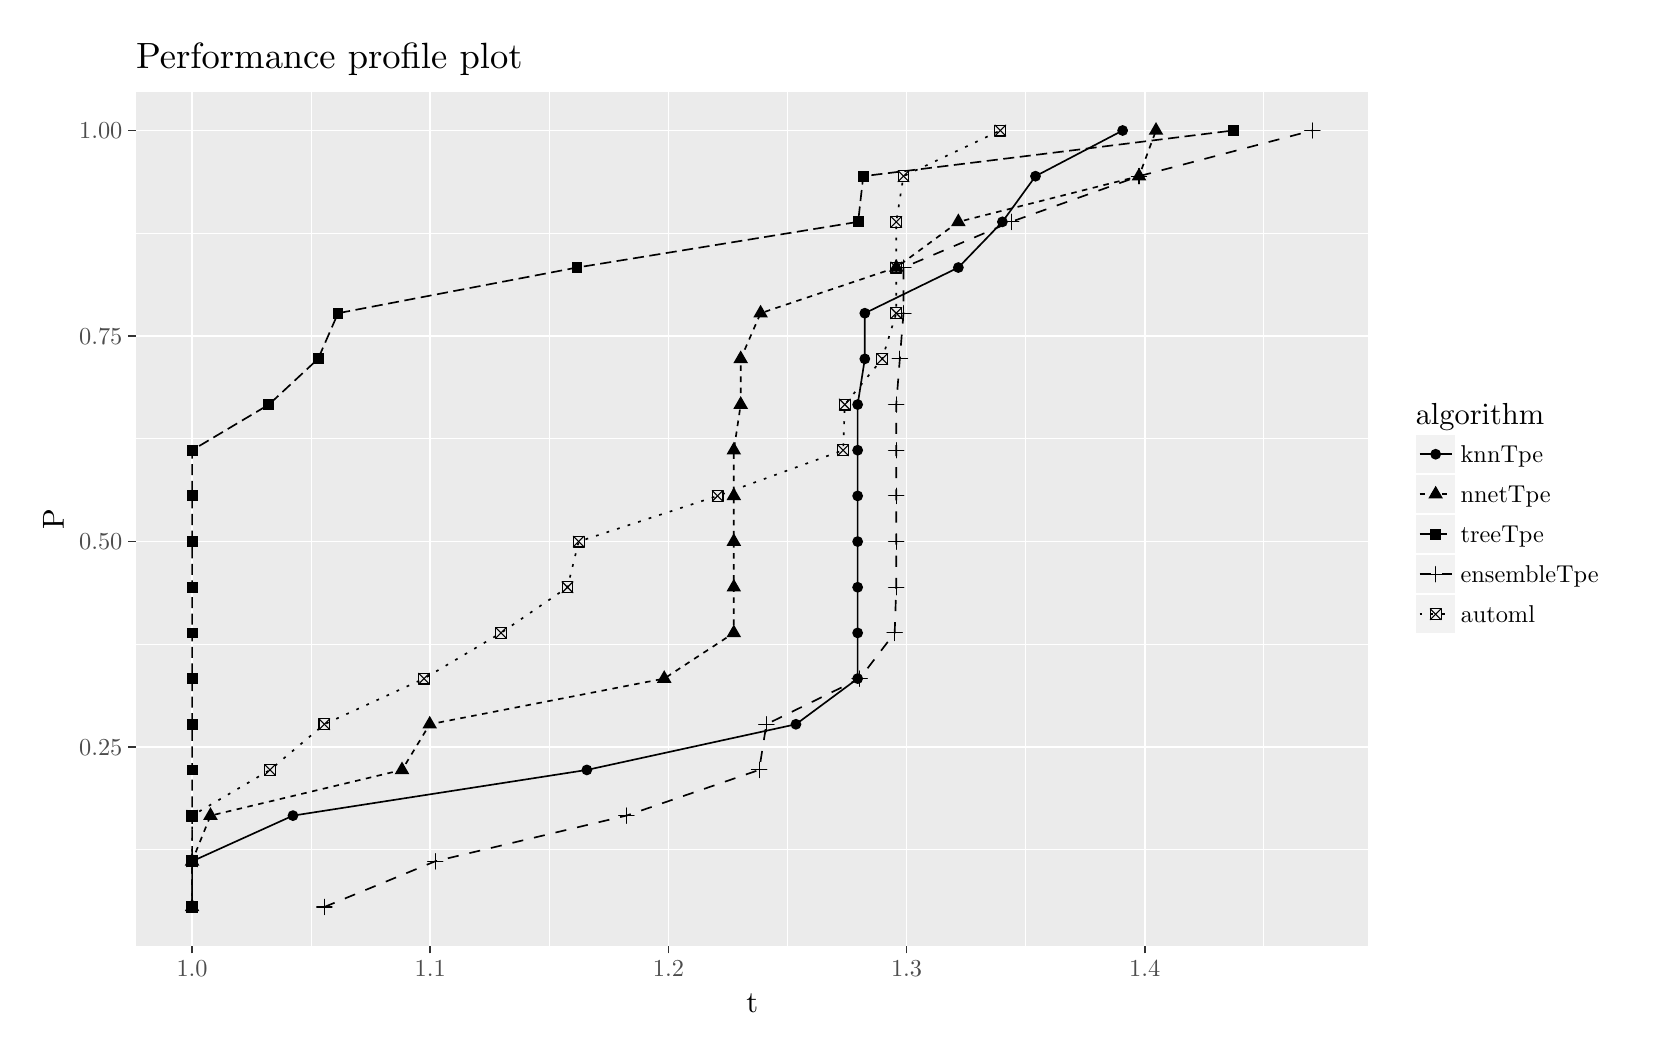
\begin{tikzpicture}[x=1pt,y=1pt]
\definecolor{fillColor}{RGB}{255,255,255}
\path[use as bounding box,fill=fillColor,fill opacity=0.00] (0,0) rectangle (578.16,361.35);
\begin{scope}
\path[clip] (  0.00,  0.00) rectangle (578.16,361.35);
\definecolor{drawColor}{RGB}{255,255,255}
\definecolor{fillColor}{RGB}{255,255,255}

\path[draw=drawColor,line width= 0.6pt,line join=round,line cap=round,fill=fillColor] (  0.00,  0.00) rectangle (578.16,361.35);
\end{scope}
\begin{scope}
\path[clip] ( 39.17, 29.59) rectangle (484.47,338.21);
\definecolor{fillColor}{gray}{0.92}

\path[fill=fillColor] ( 39.17, 29.59) rectangle (484.47,338.21);
\definecolor{drawColor}{RGB}{255,255,255}

\path[draw=drawColor,line width= 0.3pt,line join=round] ( 39.17, 64.25) --
	(484.47, 64.25);

\path[draw=drawColor,line width= 0.3pt,line join=round] ( 39.17,138.51) --
	(484.47,138.51);

\path[draw=drawColor,line width= 0.3pt,line join=round] ( 39.17,212.78) --
	(484.47,212.78);

\path[draw=drawColor,line width= 0.3pt,line join=round] ( 39.17,287.05) --
	(484.47,287.05);

\path[draw=drawColor,line width= 0.3pt,line join=round] (102.44, 29.59) --
	(102.44,338.21);

\path[draw=drawColor,line width= 0.3pt,line join=round] (188.50, 29.59) --
	(188.50,338.21);

\path[draw=drawColor,line width= 0.3pt,line join=round] (274.56, 29.59) --
	(274.56,338.21);

\path[draw=drawColor,line width= 0.3pt,line join=round] (360.62, 29.59) --
	(360.62,338.21);

\path[draw=drawColor,line width= 0.3pt,line join=round] (446.68, 29.59) --
	(446.68,338.21);

\path[draw=drawColor,line width= 0.6pt,line join=round] ( 39.17,101.38) --
	(484.47,101.38);

\path[draw=drawColor,line width= 0.6pt,line join=round] ( 39.17,175.65) --
	(484.47,175.65);

\path[draw=drawColor,line width= 0.6pt,line join=round] ( 39.17,249.92) --
	(484.47,249.92);

\path[draw=drawColor,line width= 0.6pt,line join=round] ( 39.17,324.19) --
	(484.47,324.19);

\path[draw=drawColor,line width= 0.6pt,line join=round] ( 59.41, 29.59) --
	( 59.41,338.21);

\path[draw=drawColor,line width= 0.6pt,line join=round] (145.47, 29.59) --
	(145.47,338.21);

\path[draw=drawColor,line width= 0.6pt,line join=round] (231.53, 29.59) --
	(231.53,338.21);

\path[draw=drawColor,line width= 0.6pt,line join=round] (317.59, 29.59) --
	(317.59,338.21);

\path[draw=drawColor,line width= 0.6pt,line join=round] (403.65, 29.59) --
	(403.65,338.21);
\definecolor{drawColor}{RGB}{0,0,0}

\path[draw=drawColor,line width= 0.6pt,line join=round] ( 59.41, 43.62) --
	( 59.41, 60.12) --
	( 95.86, 76.62) --
	(202.06, 93.13) --
	(277.61,109.63) --
	(299.91,126.14) --
	(299.91,142.64) --
	(299.91,159.14) --
	(299.91,175.65) --
	(299.91,192.15) --
	(299.91,208.66) --
	(299.91,225.16) --
	(302.50,241.67) --
	(302.50,258.17) --
	(336.30,274.67) --
	(352.21,291.18) --
	(364.17,307.68) --
	(395.66,324.19);

\path[draw=drawColor,line width= 0.6pt,dash pattern=on 2pt off 2pt ,line join=round] ( 59.41, 43.62) --
	( 59.41, 60.12) --
	( 66.06, 76.62) --
	(135.27, 93.13) --
	(145.28,109.63) --
	(230.01,126.14) --
	(255.16,142.64) --
	(255.16,159.14) --
	(255.16,175.65) --
	(255.16,192.15) --
	(255.16,208.66) --
	(257.65,225.16) --
	(257.65,241.67) --
	(264.84,258.17) --
	(313.85,274.67) --
	(336.30,291.18) --
	(401.58,307.68) --
	(407.72,324.19);

\path[draw=drawColor,line width= 0.6pt,dash pattern=on 4pt off 2pt ,line join=round] ( 59.41, 43.62) --
	( 59.41, 60.12) --
	( 59.41, 76.62) --
	( 59.41, 93.13) --
	( 59.41,109.63) --
	( 59.41,126.14) --
	( 59.41,142.64) --
	( 59.41,159.14) --
	( 59.41,175.65) --
	( 59.41,192.15) --
	( 59.41,208.66) --
	( 87.17,225.16) --
	(104.94,241.67) --
	(112.15,258.17) --
	(198.50,274.67) --
	(300.08,291.18) --
	(301.93,307.68) --
	(435.58,324.19);

\path[draw=drawColor,line width= 0.6pt,dash pattern=on 4pt off 4pt ,line join=round] (107.22, 43.62) --
	(147.27, 60.12) --
	(216.33, 76.62) --
	(264.31, 93.13) --
	(266.93,109.63) --
	(300.64,126.14) --
	(313.29,142.64) --
	(313.85,159.14) --
	(313.85,175.65) --
	(313.85,192.15) --
	(313.85,208.66) --
	(313.85,225.16) --
	(315.15,241.67) --
	(316.47,258.17) --
	(316.47,274.67) --
	(355.35,291.18) --
	(401.58,307.68) --
	(464.23,324.19);

\path[draw=drawColor,line width= 0.6pt,dash pattern=on 1pt off 3pt ,line join=round] ( 59.41, 43.62) --
	( 59.41, 60.12) --
	( 59.41, 76.62) --
	( 87.56, 93.13) --
	(107.22,109.63) --
	(143.22,126.14) --
	(171.03,142.64) --
	(195.06,159.14) --
	(199.09,175.65) --
	(249.29,192.15) --
	(294.68,208.66) --
	(295.26,225.16) --
	(308.80,241.67) --
	(313.85,258.17) --
	(313.85,274.67) --
	(313.85,291.18) --
	(316.47,307.68) --
	(351.46,324.19);
\definecolor{fillColor}{RGB}{0,0,0}

\path[fill=fillColor] ( 59.41, 43.62) circle (  1.96);

\path[fill=fillColor] ( 59.41, 60.12) circle (  1.96);

\path[fill=fillColor] ( 95.86, 76.62) circle (  1.96);

\path[fill=fillColor] (202.06, 93.13) circle (  1.96);

\path[fill=fillColor] (277.61,109.63) circle (  1.96);

\path[fill=fillColor] (299.91,126.14) circle (  1.96);

\path[fill=fillColor] (299.91,142.64) circle (  1.96);

\path[fill=fillColor] (299.91,159.14) circle (  1.96);

\path[fill=fillColor] (299.91,175.65) circle (  1.96);

\path[fill=fillColor] (299.91,192.15) circle (  1.96);

\path[fill=fillColor] (299.91,208.66) circle (  1.96);

\path[fill=fillColor] (299.91,225.16) circle (  1.96);

\path[fill=fillColor] (302.50,241.67) circle (  1.96);

\path[fill=fillColor] (302.50,258.17) circle (  1.96);

\path[fill=fillColor] (336.30,274.67) circle (  1.96);

\path[fill=fillColor] (352.21,291.18) circle (  1.96);

\path[fill=fillColor] (364.17,307.68) circle (  1.96);

\path[fill=fillColor] (395.66,324.19) circle (  1.96);

\path[fill=fillColor] ( 59.41, 46.67) --
	( 62.05, 42.09) --
	( 56.77, 42.09) --
	cycle;

\path[fill=fillColor] ( 59.41, 63.17) --
	( 62.05, 58.59) --
	( 56.77, 58.59) --
	cycle;

\path[fill=fillColor] ( 66.06, 79.67) --
	( 68.70, 75.10) --
	( 63.42, 75.10) --
	cycle;

\path[fill=fillColor] (135.27, 96.18) --
	(137.91, 91.60) --
	(132.62, 91.60) --
	cycle;

\path[fill=fillColor] (145.28,112.68) --
	(147.92,108.11) --
	(142.64,108.11) --
	cycle;

\path[fill=fillColor] (230.01,129.19) --
	(232.65,124.61) --
	(227.37,124.61) --
	cycle;

\path[fill=fillColor] (255.16,145.69) --
	(257.80,141.11) --
	(252.52,141.11) --
	cycle;

\path[fill=fillColor] (255.16,162.20) --
	(257.80,157.62) --
	(252.52,157.62) --
	cycle;

\path[fill=fillColor] (255.16,178.70) --
	(257.80,174.12) --
	(252.52,174.12) --
	cycle;

\path[fill=fillColor] (255.16,195.20) --
	(257.80,190.63) --
	(252.52,190.63) --
	cycle;

\path[fill=fillColor] (255.16,211.71) --
	(257.80,207.13) --
	(252.52,207.13) --
	cycle;

\path[fill=fillColor] (257.65,228.21) --
	(260.29,223.64) --
	(255.00,223.64) --
	cycle;

\path[fill=fillColor] (257.65,244.72) --
	(260.29,240.14) --
	(255.00,240.14) --
	cycle;

\path[fill=fillColor] (264.84,261.22) --
	(267.48,256.64) --
	(262.20,256.64) --
	cycle;

\path[fill=fillColor] (313.85,277.73) --
	(316.49,273.15) --
	(311.20,273.15) --
	cycle;

\path[fill=fillColor] (336.30,294.23) --
	(338.94,289.65) --
	(333.66,289.65) --
	cycle;

\path[fill=fillColor] (401.58,310.73) --
	(404.22,306.16) --
	(398.93,306.16) --
	cycle;

\path[fill=fillColor] (407.72,327.24) --
	(410.36,322.66) --
	(405.07,322.66) --
	cycle;

\path[fill=fillColor] ( 57.45, 41.65) --
	( 61.37, 41.65) --
	( 61.37, 45.58) --
	( 57.45, 45.58) --
	cycle;

\path[fill=fillColor] ( 57.45, 58.16) --
	( 61.37, 58.16) --
	( 61.37, 62.08) --
	( 57.45, 62.08) --
	cycle;

\path[fill=fillColor] ( 57.45, 74.66) --
	( 61.37, 74.66) --
	( 61.37, 78.59) --
	( 57.45, 78.59) --
	cycle;

\path[fill=fillColor] ( 57.45, 91.17) --
	( 61.37, 91.17) --
	( 61.37, 95.09) --
	( 57.45, 95.09) --
	cycle;

\path[fill=fillColor] ( 57.45,107.67) --
	( 61.37,107.67) --
	( 61.37,111.59) --
	( 57.45,111.59) --
	cycle;

\path[fill=fillColor] ( 57.45,124.17) --
	( 61.37,124.17) --
	( 61.37,128.10) --
	( 57.45,128.10) --
	cycle;

\path[fill=fillColor] ( 57.45,140.68) --
	( 61.37,140.68) --
	( 61.37,144.60) --
	( 57.45,144.60) --
	cycle;

\path[fill=fillColor] ( 57.45,157.18) --
	( 61.37,157.18) --
	( 61.37,161.11) --
	( 57.45,161.11) --
	cycle;

\path[fill=fillColor] ( 57.45,173.69) --
	( 61.37,173.69) --
	( 61.37,177.61) --
	( 57.45,177.61) --
	cycle;

\path[fill=fillColor] ( 57.45,190.19) --
	( 61.37,190.19) --
	( 61.37,194.12) --
	( 57.45,194.12) --
	cycle;

\path[fill=fillColor] ( 57.45,206.69) --
	( 61.37,206.69) --
	( 61.37,210.62) --
	( 57.45,210.62) --
	cycle;

\path[fill=fillColor] ( 85.21,223.20) --
	( 89.13,223.20) --
	( 89.13,227.12) --
	( 85.21,227.12) --
	cycle;

\path[fill=fillColor] (102.98,239.70) --
	(106.90,239.70) --
	(106.90,243.63) --
	(102.98,243.63) --
	cycle;

\path[fill=fillColor] (110.18,256.21) --
	(114.11,256.21) --
	(114.11,260.13) --
	(110.18,260.13) --
	cycle;

\path[fill=fillColor] (196.54,272.71) --
	(200.47,272.71) --
	(200.47,276.64) --
	(196.54,276.64) --
	cycle;

\path[fill=fillColor] (298.12,289.22) --
	(302.05,289.22) --
	(302.05,293.14) --
	(298.12,293.14) --
	cycle;

\path[fill=fillColor] (299.97,305.72) --
	(303.89,305.72) --
	(303.89,309.64) --
	(299.97,309.64) --
	cycle;

\path[fill=fillColor] (433.62,322.22) --
	(437.54,322.22) --
	(437.54,326.15) --
	(433.62,326.15) --
	cycle;

\path[draw=drawColor,line width= 0.4pt,line join=round,line cap=round] (104.44, 43.62) -- (109.99, 43.62);

\path[draw=drawColor,line width= 0.4pt,line join=round,line cap=round] (107.22, 40.84) -- (107.22, 46.39);

\path[draw=drawColor,line width= 0.4pt,line join=round,line cap=round] (144.50, 60.12) -- (150.05, 60.12);

\path[draw=drawColor,line width= 0.4pt,line join=round,line cap=round] (147.27, 57.34) -- (147.27, 62.89);

\path[draw=drawColor,line width= 0.4pt,line join=round,line cap=round] (213.56, 76.62) -- (219.11, 76.62);

\path[draw=drawColor,line width= 0.4pt,line join=round,line cap=round] (216.33, 73.85) -- (216.33, 79.40);

\path[draw=drawColor,line width= 0.4pt,line join=round,line cap=round] (261.53, 93.13) -- (267.08, 93.13);

\path[draw=drawColor,line width= 0.4pt,line join=round,line cap=round] (264.31, 90.35) -- (264.31, 95.90);

\path[draw=drawColor,line width= 0.4pt,line join=round,line cap=round] (264.16,109.63) -- (269.71,109.63);

\path[draw=drawColor,line width= 0.4pt,line join=round,line cap=round] (266.93,106.86) -- (266.93,112.41);

\path[draw=drawColor,line width= 0.4pt,line join=round,line cap=round] (297.86,126.14) -- (303.41,126.14);

\path[draw=drawColor,line width= 0.4pt,line join=round,line cap=round] (300.64,123.36) -- (300.64,128.91);

\path[draw=drawColor,line width= 0.4pt,line join=round,line cap=round] (310.52,142.64) -- (316.07,142.64);

\path[draw=drawColor,line width= 0.4pt,line join=round,line cap=round] (313.29,139.87) -- (313.29,145.42);

\path[draw=drawColor,line width= 0.4pt,line join=round,line cap=round] (311.07,159.14) -- (316.62,159.14);

\path[draw=drawColor,line width= 0.4pt,line join=round,line cap=round] (313.85,156.37) -- (313.85,161.92);

\path[draw=drawColor,line width= 0.4pt,line join=round,line cap=round] (311.07,175.65) -- (316.62,175.65);

\path[draw=drawColor,line width= 0.4pt,line join=round,line cap=round] (313.85,172.87) -- (313.85,178.42);

\path[draw=drawColor,line width= 0.4pt,line join=round,line cap=round] (311.07,192.15) -- (316.62,192.15);

\path[draw=drawColor,line width= 0.4pt,line join=round,line cap=round] (313.85,189.38) -- (313.85,194.93);

\path[draw=drawColor,line width= 0.4pt,line join=round,line cap=round] (311.07,208.66) -- (316.62,208.66);

\path[draw=drawColor,line width= 0.4pt,line join=round,line cap=round] (313.85,205.88) -- (313.85,211.43);

\path[draw=drawColor,line width= 0.4pt,line join=round,line cap=round] (311.07,225.16) -- (316.62,225.16);

\path[draw=drawColor,line width= 0.4pt,line join=round,line cap=round] (313.85,222.39) -- (313.85,227.94);

\path[draw=drawColor,line width= 0.4pt,line join=round,line cap=round] (312.38,241.67) -- (317.93,241.67);

\path[draw=drawColor,line width= 0.4pt,line join=round,line cap=round] (315.15,238.89) -- (315.15,244.44);

\path[draw=drawColor,line width= 0.4pt,line join=round,line cap=round] (313.70,258.17) -- (319.25,258.17);

\path[draw=drawColor,line width= 0.4pt,line join=round,line cap=round] (316.47,255.39) -- (316.47,260.94);

\path[draw=drawColor,line width= 0.4pt,line join=round,line cap=round] (313.70,274.67) -- (319.25,274.67);

\path[draw=drawColor,line width= 0.4pt,line join=round,line cap=round] (316.47,271.90) -- (316.47,277.45);

\path[draw=drawColor,line width= 0.4pt,line join=round,line cap=round] (352.57,291.18) -- (358.12,291.18);

\path[draw=drawColor,line width= 0.4pt,line join=round,line cap=round] (355.35,288.40) -- (355.35,293.95);

\path[draw=drawColor,line width= 0.4pt,line join=round,line cap=round] (398.80,307.68) -- (404.35,307.68);

\path[draw=drawColor,line width= 0.4pt,line join=round,line cap=round] (401.58,304.91) -- (401.58,310.46);

\path[draw=drawColor,line width= 0.4pt,line join=round,line cap=round] (461.45,324.19) -- (467.00,324.19);

\path[draw=drawColor,line width= 0.4pt,line join=round,line cap=round] (464.23,321.41) -- (464.23,326.96);

\path[draw=drawColor,line width= 0.4pt,line join=round,line cap=round] ( 57.45, 41.65) rectangle ( 61.37, 45.58);

\path[draw=drawColor,line width= 0.4pt,line join=round,line cap=round] ( 57.45, 41.65) -- ( 61.37, 45.58);

\path[draw=drawColor,line width= 0.4pt,line join=round,line cap=round] ( 57.45, 45.58) -- ( 61.37, 41.65);

\path[draw=drawColor,line width= 0.4pt,line join=round,line cap=round] ( 57.45, 58.16) rectangle ( 61.37, 62.08);

\path[draw=drawColor,line width= 0.4pt,line join=round,line cap=round] ( 57.45, 58.16) -- ( 61.37, 62.08);

\path[draw=drawColor,line width= 0.4pt,line join=round,line cap=round] ( 57.45, 62.08) -- ( 61.37, 58.16);

\path[draw=drawColor,line width= 0.4pt,line join=round,line cap=round] ( 57.45, 74.66) rectangle ( 61.37, 78.59);

\path[draw=drawColor,line width= 0.4pt,line join=round,line cap=round] ( 57.45, 74.66) -- ( 61.37, 78.59);

\path[draw=drawColor,line width= 0.4pt,line join=round,line cap=round] ( 57.45, 78.59) -- ( 61.37, 74.66);

\path[draw=drawColor,line width= 0.4pt,line join=round,line cap=round] ( 85.60, 91.17) rectangle ( 89.52, 95.09);

\path[draw=drawColor,line width= 0.4pt,line join=round,line cap=round] ( 85.60, 91.17) -- ( 89.52, 95.09);

\path[draw=drawColor,line width= 0.4pt,line join=round,line cap=round] ( 85.60, 95.09) -- ( 89.52, 91.17);

\path[draw=drawColor,line width= 0.4pt,line join=round,line cap=round] (105.26,107.67) rectangle (109.18,111.59);

\path[draw=drawColor,line width= 0.4pt,line join=round,line cap=round] (105.26,107.67) -- (109.18,111.59);

\path[draw=drawColor,line width= 0.4pt,line join=round,line cap=round] (105.26,111.59) -- (109.18,107.67);

\path[draw=drawColor,line width= 0.4pt,line join=round,line cap=round] (141.25,124.17) rectangle (145.18,128.10);

\path[draw=drawColor,line width= 0.4pt,line join=round,line cap=round] (141.25,124.17) -- (145.18,128.10);

\path[draw=drawColor,line width= 0.4pt,line join=round,line cap=round] (141.25,128.10) -- (145.18,124.17);

\path[draw=drawColor,line width= 0.4pt,line join=round,line cap=round] (169.07,140.68) rectangle (172.99,144.60);

\path[draw=drawColor,line width= 0.4pt,line join=round,line cap=round] (169.07,140.68) -- (172.99,144.60);

\path[draw=drawColor,line width= 0.4pt,line join=round,line cap=round] (169.07,144.60) -- (172.99,140.68);

\path[draw=drawColor,line width= 0.4pt,line join=round,line cap=round] (193.10,157.18) rectangle (197.02,161.11);

\path[draw=drawColor,line width= 0.4pt,line join=round,line cap=round] (193.10,157.18) -- (197.02,161.11);

\path[draw=drawColor,line width= 0.4pt,line join=round,line cap=round] (193.10,161.11) -- (197.02,157.18);

\path[draw=drawColor,line width= 0.4pt,line join=round,line cap=round] (197.13,173.69) rectangle (201.05,177.61);

\path[draw=drawColor,line width= 0.4pt,line join=round,line cap=round] (197.13,173.69) -- (201.05,177.61);

\path[draw=drawColor,line width= 0.4pt,line join=round,line cap=round] (197.13,177.61) -- (201.05,173.69);

\path[draw=drawColor,line width= 0.4pt,line join=round,line cap=round] (247.33,190.19) rectangle (251.25,194.12);

\path[draw=drawColor,line width= 0.4pt,line join=round,line cap=round] (247.33,190.19) -- (251.25,194.12);

\path[draw=drawColor,line width= 0.4pt,line join=round,line cap=round] (247.33,194.12) -- (251.25,190.19);

\path[draw=drawColor,line width= 0.4pt,line join=round,line cap=round] (292.71,206.69) rectangle (296.64,210.62);

\path[draw=drawColor,line width= 0.4pt,line join=round,line cap=round] (292.71,206.69) -- (296.64,210.62);

\path[draw=drawColor,line width= 0.4pt,line join=round,line cap=round] (292.71,210.62) -- (296.64,206.69);

\path[draw=drawColor,line width= 0.4pt,line join=round,line cap=round] (293.30,223.20) rectangle (297.23,227.12);

\path[draw=drawColor,line width= 0.4pt,line join=round,line cap=round] (293.30,223.20) -- (297.23,227.12);

\path[draw=drawColor,line width= 0.4pt,line join=round,line cap=round] (293.30,227.12) -- (297.23,223.20);

\path[draw=drawColor,line width= 0.4pt,line join=round,line cap=round] (306.84,239.70) rectangle (310.77,243.63);

\path[draw=drawColor,line width= 0.4pt,line join=round,line cap=round] (306.84,239.70) -- (310.77,243.63);

\path[draw=drawColor,line width= 0.4pt,line join=round,line cap=round] (306.84,243.63) -- (310.77,239.70);

\path[draw=drawColor,line width= 0.4pt,line join=round,line cap=round] (311.89,256.21) rectangle (315.81,260.13);

\path[draw=drawColor,line width= 0.4pt,line join=round,line cap=round] (311.89,256.21) -- (315.81,260.13);

\path[draw=drawColor,line width= 0.4pt,line join=round,line cap=round] (311.89,260.13) -- (315.81,256.21);

\path[draw=drawColor,line width= 0.4pt,line join=round,line cap=round] (311.89,272.71) rectangle (315.81,276.64);

\path[draw=drawColor,line width= 0.4pt,line join=round,line cap=round] (311.89,272.71) -- (315.81,276.64);

\path[draw=drawColor,line width= 0.4pt,line join=round,line cap=round] (311.89,276.64) -- (315.81,272.71);

\path[draw=drawColor,line width= 0.4pt,line join=round,line cap=round] (311.89,289.22) rectangle (315.81,293.14);

\path[draw=drawColor,line width= 0.4pt,line join=round,line cap=round] (311.89,289.22) -- (315.81,293.14);

\path[draw=drawColor,line width= 0.4pt,line join=round,line cap=round] (311.89,293.14) -- (315.81,289.22);

\path[draw=drawColor,line width= 0.4pt,line join=round,line cap=round] (314.51,305.72) rectangle (318.43,309.64);

\path[draw=drawColor,line width= 0.4pt,line join=round,line cap=round] (314.51,305.72) -- (318.43,309.64);

\path[draw=drawColor,line width= 0.4pt,line join=round,line cap=round] (314.51,309.64) -- (318.43,305.72);

\path[draw=drawColor,line width= 0.4pt,line join=round,line cap=round] (349.50,322.22) rectangle (353.42,326.15);

\path[draw=drawColor,line width= 0.4pt,line join=round,line cap=round] (349.50,322.22) -- (353.42,326.15);

\path[draw=drawColor,line width= 0.4pt,line join=round,line cap=round] (349.50,326.15) -- (353.42,322.22);
\end{scope}
\begin{scope}
\path[clip] (  0.00,  0.00) rectangle (578.16,361.35);
\definecolor{drawColor}{gray}{0.30}

\node[text=drawColor,anchor=base east,inner sep=0pt, outer sep=0pt, scale=  0.88] at ( 34.22, 98.35) {0.25};

\node[text=drawColor,anchor=base east,inner sep=0pt, outer sep=0pt, scale=  0.88] at ( 34.22,172.62) {0.50};

\node[text=drawColor,anchor=base east,inner sep=0pt, outer sep=0pt, scale=  0.88] at ( 34.22,246.89) {0.75};

\node[text=drawColor,anchor=base east,inner sep=0pt, outer sep=0pt, scale=  0.88] at ( 34.22,321.16) {1.00};
\end{scope}
\begin{scope}
\path[clip] (  0.00,  0.00) rectangle (578.16,361.35);
\definecolor{drawColor}{gray}{0.20}

\path[draw=drawColor,line width= 0.6pt,line join=round] ( 36.42,101.38) --
	( 39.17,101.38);

\path[draw=drawColor,line width= 0.6pt,line join=round] ( 36.42,175.65) --
	( 39.17,175.65);

\path[draw=drawColor,line width= 0.6pt,line join=round] ( 36.42,249.92) --
	( 39.17,249.92);

\path[draw=drawColor,line width= 0.6pt,line join=round] ( 36.42,324.19) --
	( 39.17,324.19);
\end{scope}
\begin{scope}
\path[clip] (  0.00,  0.00) rectangle (578.16,361.35);
\definecolor{drawColor}{gray}{0.20}

\path[draw=drawColor,line width= 0.6pt,line join=round] ( 59.41, 26.84) --
	( 59.41, 29.59);

\path[draw=drawColor,line width= 0.6pt,line join=round] (145.47, 26.84) --
	(145.47, 29.59);

\path[draw=drawColor,line width= 0.6pt,line join=round] (231.53, 26.84) --
	(231.53, 29.59);

\path[draw=drawColor,line width= 0.6pt,line join=round] (317.59, 26.84) --
	(317.59, 29.59);

\path[draw=drawColor,line width= 0.6pt,line join=round] (403.65, 26.84) --
	(403.65, 29.59);
\end{scope}
\begin{scope}
\path[clip] (  0.00,  0.00) rectangle (578.16,361.35);
\definecolor{drawColor}{gray}{0.30}

\node[text=drawColor,anchor=base,inner sep=0pt, outer sep=0pt, scale=  0.88] at ( 59.41, 18.58) {1.0};

\node[text=drawColor,anchor=base,inner sep=0pt, outer sep=0pt, scale=  0.88] at (145.47, 18.58) {1.1};

\node[text=drawColor,anchor=base,inner sep=0pt, outer sep=0pt, scale=  0.88] at (231.53, 18.58) {1.2};

\node[text=drawColor,anchor=base,inner sep=0pt, outer sep=0pt, scale=  0.88] at (317.59, 18.58) {1.3};

\node[text=drawColor,anchor=base,inner sep=0pt, outer sep=0pt, scale=  0.88] at (403.65, 18.58) {1.4};
\end{scope}
\begin{scope}
\path[clip] (  0.00,  0.00) rectangle (578.16,361.35);
\definecolor{drawColor}{RGB}{0,0,0}

\node[text=drawColor,anchor=base,inner sep=0pt, outer sep=0pt, scale=  1.10] at (261.82,  5.50) {t};
\end{scope}
\begin{scope}
\path[clip] (  0.00,  0.00) rectangle (578.16,361.35);
\definecolor{drawColor}{RGB}{0,0,0}

\node[text=drawColor,rotate= 90.00,anchor=base,inner sep=0pt, outer sep=0pt, scale=  1.10] at ( 13.08,183.90) {P};
\end{scope}
\begin{scope}
\path[clip] (  0.00,  0.00) rectangle (578.16,361.35);
\definecolor{fillColor}{RGB}{255,255,255}

\path[fill=fillColor] (495.85,136.48) rectangle (572.66,231.32);
\end{scope}
\begin{scope}
\path[clip] (  0.00,  0.00) rectangle (578.16,361.35);
\definecolor{drawColor}{RGB}{0,0,0}

\node[text=drawColor,anchor=base west,inner sep=0pt, outer sep=0pt, scale=  1.10] at (501.54,218.05) {algorithm};
\end{scope}
\begin{scope}
\path[clip] (  0.00,  0.00) rectangle (578.16,361.35);
\definecolor{drawColor}{RGB}{255,255,255}
\definecolor{fillColor}{gray}{0.95}

\path[draw=drawColor,line width= 0.6pt,line join=round,line cap=round,fill=fillColor] (501.54,199.99) rectangle (515.99,214.44);
\end{scope}
\begin{scope}
\path[clip] (  0.00,  0.00) rectangle (578.16,361.35);
\definecolor{drawColor}{RGB}{0,0,0}

\path[draw=drawColor,line width= 0.6pt,line join=round] (502.98,207.21) -- (514.55,207.21);
\end{scope}
\begin{scope}
\path[clip] (  0.00,  0.00) rectangle (578.16,361.35);
\definecolor{fillColor}{RGB}{0,0,0}

\path[fill=fillColor] (508.77,207.21) circle (  1.96);
\end{scope}
\begin{scope}
\path[clip] (  0.00,  0.00) rectangle (578.16,361.35);
\definecolor{drawColor}{RGB}{255,255,255}
\definecolor{fillColor}{gray}{0.95}

\path[draw=drawColor,line width= 0.6pt,line join=round,line cap=round,fill=fillColor] (501.54,185.53) rectangle (515.99,199.99);
\end{scope}
\begin{scope}
\path[clip] (  0.00,  0.00) rectangle (578.16,361.35);
\definecolor{drawColor}{RGB}{0,0,0}

\path[draw=drawColor,line width= 0.6pt,dash pattern=on 2pt off 2pt ,line join=round] (502.98,192.76) -- (514.55,192.76);
\end{scope}
\begin{scope}
\path[clip] (  0.00,  0.00) rectangle (578.16,361.35);
\definecolor{fillColor}{RGB}{0,0,0}

\path[fill=fillColor] (508.77,195.81) --
	(511.41,191.23) --
	(506.12,191.23) --
	cycle;
\end{scope}
\begin{scope}
\path[clip] (  0.00,  0.00) rectangle (578.16,361.35);
\definecolor{drawColor}{RGB}{255,255,255}
\definecolor{fillColor}{gray}{0.95}

\path[draw=drawColor,line width= 0.6pt,line join=round,line cap=round,fill=fillColor] (501.54,171.08) rectangle (515.99,185.53);
\end{scope}
\begin{scope}
\path[clip] (  0.00,  0.00) rectangle (578.16,361.35);
\definecolor{drawColor}{RGB}{0,0,0}

\path[draw=drawColor,line width= 0.6pt,dash pattern=on 4pt off 2pt ,line join=round] (502.98,178.31) -- (514.55,178.31);
\end{scope}
\begin{scope}
\path[clip] (  0.00,  0.00) rectangle (578.16,361.35);
\definecolor{fillColor}{RGB}{0,0,0}

\path[fill=fillColor] (506.80,176.34) --
	(510.73,176.34) --
	(510.73,180.27) --
	(506.80,180.27) --
	cycle;
\end{scope}
\begin{scope}
\path[clip] (  0.00,  0.00) rectangle (578.16,361.35);
\definecolor{drawColor}{RGB}{255,255,255}
\definecolor{fillColor}{gray}{0.95}

\path[draw=drawColor,line width= 0.6pt,line join=round,line cap=round,fill=fillColor] (501.54,156.63) rectangle (515.99,171.08);
\end{scope}
\begin{scope}
\path[clip] (  0.00,  0.00) rectangle (578.16,361.35);
\definecolor{drawColor}{RGB}{0,0,0}

\path[draw=drawColor,line width= 0.6pt,dash pattern=on 4pt off 4pt ,line join=round] (502.98,163.85) -- (514.55,163.85);
\end{scope}
\begin{scope}
\path[clip] (  0.00,  0.00) rectangle (578.16,361.35);
\definecolor{drawColor}{RGB}{0,0,0}

\path[draw=drawColor,line width= 0.4pt,line join=round,line cap=round] (505.99,163.85) -- (511.54,163.85);

\path[draw=drawColor,line width= 0.4pt,line join=round,line cap=round] (508.77,161.08) -- (508.77,166.63);
\end{scope}
\begin{scope}
\path[clip] (  0.00,  0.00) rectangle (578.16,361.35);
\definecolor{drawColor}{RGB}{255,255,255}
\definecolor{fillColor}{gray}{0.95}

\path[draw=drawColor,line width= 0.6pt,line join=round,line cap=round,fill=fillColor] (501.54,142.17) rectangle (515.99,156.63);
\end{scope}
\begin{scope}
\path[clip] (  0.00,  0.00) rectangle (578.16,361.35);
\definecolor{drawColor}{RGB}{0,0,0}

\path[draw=drawColor,line width= 0.6pt,dash pattern=on 1pt off 3pt ,line join=round] (502.98,149.40) -- (514.55,149.40);
\end{scope}
\begin{scope}
\path[clip] (  0.00,  0.00) rectangle (578.16,361.35);
\definecolor{drawColor}{RGB}{0,0,0}

\path[draw=drawColor,line width= 0.4pt,line join=round,line cap=round] (506.80,147.44) rectangle (510.73,151.36);

\path[draw=drawColor,line width= 0.4pt,line join=round,line cap=round] (506.80,147.44) -- (510.73,151.36);

\path[draw=drawColor,line width= 0.4pt,line join=round,line cap=round] (506.80,151.36) -- (510.73,147.44);
\end{scope}
\begin{scope}
\path[clip] (  0.00,  0.00) rectangle (578.16,361.35);
\definecolor{drawColor}{RGB}{0,0,0}

\node[text=drawColor,anchor=base west,inner sep=0pt, outer sep=0pt, scale=  0.88] at (517.80,204.18) {knnTpe};
\end{scope}
\begin{scope}
\path[clip] (  0.00,  0.00) rectangle (578.16,361.35);
\definecolor{drawColor}{RGB}{0,0,0}

\node[text=drawColor,anchor=base west,inner sep=0pt, outer sep=0pt, scale=  0.88] at (517.80,189.73) {nnetTpe};
\end{scope}
\begin{scope}
\path[clip] (  0.00,  0.00) rectangle (578.16,361.35);
\definecolor{drawColor}{RGB}{0,0,0}

\node[text=drawColor,anchor=base west,inner sep=0pt, outer sep=0pt, scale=  0.88] at (517.80,175.28) {treeTpe};
\end{scope}
\begin{scope}
\path[clip] (  0.00,  0.00) rectangle (578.16,361.35);
\definecolor{drawColor}{RGB}{0,0,0}

\node[text=drawColor,anchor=base west,inner sep=0pt, outer sep=0pt, scale=  0.88] at (517.80,160.82) {ensembleTpe};
\end{scope}
\begin{scope}
\path[clip] (  0.00,  0.00) rectangle (578.16,361.35);
\definecolor{drawColor}{RGB}{0,0,0}

\node[text=drawColor,anchor=base west,inner sep=0pt, outer sep=0pt, scale=  0.88] at (517.80,146.37) {automl};
\end{scope}
\begin{scope}
\path[clip] (  0.00,  0.00) rectangle (578.16,361.35);
\definecolor{drawColor}{RGB}{0,0,0}

\node[text=drawColor,anchor=base west,inner sep=0pt, outer sep=0pt, scale=  1.32] at ( 39.17,346.76) {Performance profile plot};
\end{scope}
\end{tikzpicture}

